\subsubsection*{Creación de nuestra CA en Docker}

La estrategia para crear nuestra CA será seguir los pasos que se deberían realizar en un servidor 
habitual, pero partiendo desde una imagen de Docker de Ubuntu (de stock), y luego realizando un 
commit de estas configuraciones. Luego, archivos importantes como el el certificado root y la llave
privada deberán resguardarse, o simplemente resguardar el contenedor creado. 

Se utilizó esta estrategia ya que no había imágenes oficiales que nos sirva para tal fin, por el 
simple hecho de que únicamente se requiere tener instalado OpenSSL y tenerlo configurado.

\noindent Como primer paso, corremos una imagen del sistema operativo Ubuntu

\begin{verbatim}
    docker run -it -v $PWD/ca:/root/ca ubuntu
\end{verbatim}

\noindent Dentro del contenedor, ejecutamos los siguientes comandos:
\begin{verbatim}
    apt-get update
    apt-get install ntp
    apt-get install openssl
\end{verbatim}

\noindent Establecer el hostname al contenedor, hay una linea con la ip del contenedor y el nombre del mismo, 
que es utilizado como hostname, en nuestro caso
\begin{verbatim}
    172.17.0.2      080dec560726
\end{verbatim}

\noindent Lo cambiamos por un hostname con el dominio incluido
\begin{verbatim}
    172.17.0.2      ca.salvadorcatalfamo.intra
\end{verbatim}

\noindent Creamos las carpetas para mejor organización
\begin{verbatim}
    mkdir /root/newcerts
    mkdir /root/certs
    mkdir /root/crl
    mkdir /root/private
    mkdir /root/requests
\end{verbatim}

\noindent Creamos un archivo vacío y un archivo que contiene el primer numero de serie para los certificados 
\begin{verbatim}
    touch index.txt
    echo '1234' > serial
\end{verbatim}

\noindent Luego hay que crear la llave privada y el certificado root, en este caso nos pedirá una contraseña, si este servidor 
se usará en un ambiente de producción, deberá ser una contraseña compleja.

\begin{verbatim}
    openssl genrsa -aes256 -out private/cakey.pem

\end{verbatim}

\noindent Una vez que generamos la llave privada, la misma será utilizada como entrada en la creación de 
nuestro certificado root. Nos pedirá algunos datos de localización y relacionados a la 
organización

\begin{verbatim}
    openssl req -new -x509 -key /root/ca/private/cakey.pem -out cacert.pem -days 3650
\end{verbatim}

\noindent Cambiamos los permisos de los archivos que creamos
\begin{verbatim}
    chmod 600 -R /root/ca
\end{verbatim}

\noindent Realizamos unas modificaciones en el archivo de configuración, donde indicaremos 
la dirección de los certificados, y algunas opciones de configuración adicionales
\begin{verbatim}
    vim /usr/lib/ssl/openssl.cnf
\end{verbatim}

Una vez que realizamos estos pasos, estamos listos para realizar el commit de la imagen, con esto,
todos los pasos que realizamos (instalar los paquetes, modificar los archivos de configuración, etc)
no son necesarios que se ejecuten nuevamente.

Para realizar un commit, y que nuestro contenedor sea fácilmente identificable, deberemos seguir 
los siguientes pasos

\begin{verbatim}
    docker ps -a        #identificamos el último contenedor utilizado
    docker commit {id_del_contenedor} 
    docker image ls     #Identificamos la imagen recién creada
                        #no tendrá ni repositorio ni tag
    docker image tag {id_de_imagen} ca:1.0  #nombramos nuestra imagen
\end{verbatim}




Ahora cada vez que queramos correr nuestra CA, lo haremos de la siguiente manera:
\begin{verbatim}
    docker run -it -v $PWD/ca:/root/ca ca:1.0
\end{verbatim}

Em el comando anterior, estamos asumiendo que queremos compartir los archivos de la CA con el servidor 
host.

 

\subsubsection*{Nginx con Docker}

Para probar nuestro certificado, utilizaremos una imagen oficial de Nginx, 
los archivos de configuración
son los siguientes:


\begin{verbatim}
docker-compose.yml

web:
  image: nginx
  volumes:
   - ./pagina1:/usr/share/nginx/html:ro
  ports:
   - "80:80"
  environment:
   - NGINX_HOST=pagina1.salvadorcatalfamo.intra
   - NGINX_PORT=80
\end{verbatim}

En el archivo mostrado, le decimos a Docker que utilice la imagen Nginx, 
que nuestros archivos fuentes
van a estar en el directorio \textit{./pagina1} y que exponga el puerto 80, entre otras
 cosas.

\noindent Para ejecutar este contenedor, se debe ejecutar el siguiente comando:

\begin{verbatim}
    docker-compose up -d
\end{verbatim}




\subsubsection*{Creando nuestro certificado}

Para firmar un certificado, tenemos que seguir los pasos mostrados en la figura \ref{figSolCert}
: el servidor donde se alojará la web debe realizar una solicitud, 
luego nuestra CA retornará el certificado firmado. Desde el servidor web en cuestión, se debe 
crear una llave privada privada:

\begin{verbatim}
    openssl genrsa -aes256 -out pagina1.pem 2048
\end{verbatim}

\noindent Luego, se deberá crear la solicitud de firma de certificado:
\begin{verbatim}
    openssl req -new -key pagina1.pem -out pagina1.csr
\end{verbatim}

\noindent Luego enviamos esta solicitud y la firmamos en nuestra CA, esta solicitud la vamos a colocar 
en el directorio /root/ca/requests
\begin{verbatim}
    openssl ca -in pagina1.csr -out pagina1.crt
\end{verbatim}

\subsubsection*{Configuración del certificado en el servidor web}
Una vez que tenemos este certificado, lo colocamos en en el servidor web y 
lo configuramos. Para el caso de Nginx, se debe editar el archivo de configuración 
correspondiente a nuestra web, que en este caso es “pagina1.salvadorcatalfamo.intra”
con el fin de que el mismo pueda localizar correctamente los certificados firmados recientemente.
Adicionalmente, se puede obligar a que cada requerimiento sea redirigido a una conexión
segura mediante SSL.

Como se puede ver en la figura \ref{figCAdesc}, aunque el certificado esté configurado, 
el mismo no es confiable ya que nuestra entidad certificante no está importada a nuestro almacén 
local.

\begin{center}
    \begin{figure}   
       \begin{center}
          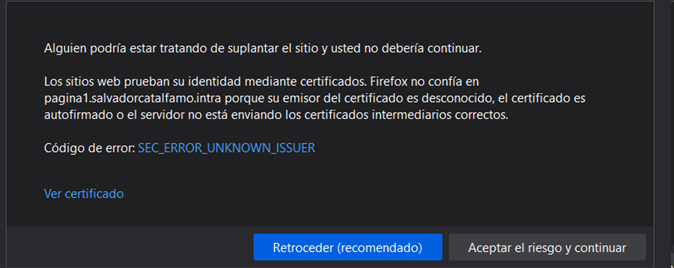
\includegraphics[width=15cm,height=6cm]{adv-2.png}
       \end{center}
       \caption{CA Desconocida}
       \label{figCAdesc}
    \end{figure}
 \end{center}

Luego de establecer en nuestra computadora (particularmente en el navegador Mozilla) que la 
entidad certificante creada es confiable, es posible ver que nuestra conexión es segura, como 
se muestra en la captura.

\begin{center}
    \begin{figure}   
       \begin{center}
          \includegraphics[width=15cm,height=7.5cm]{ca-HTTPS.png}
       \end{center}
       \caption{Resultado de la solución}
    \end{figure}
 \end{center}





